\documentclass{article}

\usepackage{../preamble}
\standalonetrue

\pagestyle{fancy}
\fancyhf{}
\rhead{Section \thesection}
\lhead{PHYS 304 Lecture 18}
\rfoot{Page \thepage}


\title{PHYS 304 Lecture 18}
\author{Ashtan Mistal}
\date{!!!}

\begin{document}

\ifstandalone
\maketitle
\fi

\graphicspath{{./Lecture18!/}}

\section{Key review of points from last lecture}

The uncertainty principle that involves the product of the variances of two observable quantities is quite distinct from the “Energy-time” uncertainty principle.  (time is not an observable)

If two observable operators commute, then the lower limit on the product of their variances is zero.  The product of the two variances can in fact be made equal to, or arbitrarily close to zero by putting the system into one of the shared eigen states that the commuting operators must share.

If two observables do not commute, then the more you try to engineer a state with a small variance in one observable, the wider is the minimum variance in the non-commuting observable.  This can be understood qualitatively when one thinks of having to express one eigen state in one basis in terms of many eigen states of another.

If one of the two observables is the Hamiltonian (total energy), then the commutator on the right hand side is directly related to the time derivative of the expectation value of the other observable in the state being studied.  This provides a useful connection to the “Energy-time” uncertainty principle, as the variance of the other observable, divided by the time derivative of its expectation value, defines a time called $\Delta t$, that is a measure of how quickly the other parameter can change by its standard deviation (effectively how quickly there would be some observable change in that observable quantity, in that particular state).  

So long as even one system observable is changing “rapidly” for a state at some time, then necessarily there is a proportionate uncertainty in the energy one would measure for that state at that time.  Conversely, if the energy of the system has a very small variance at some time, then no other observable can be changing “rapidly” at that time.

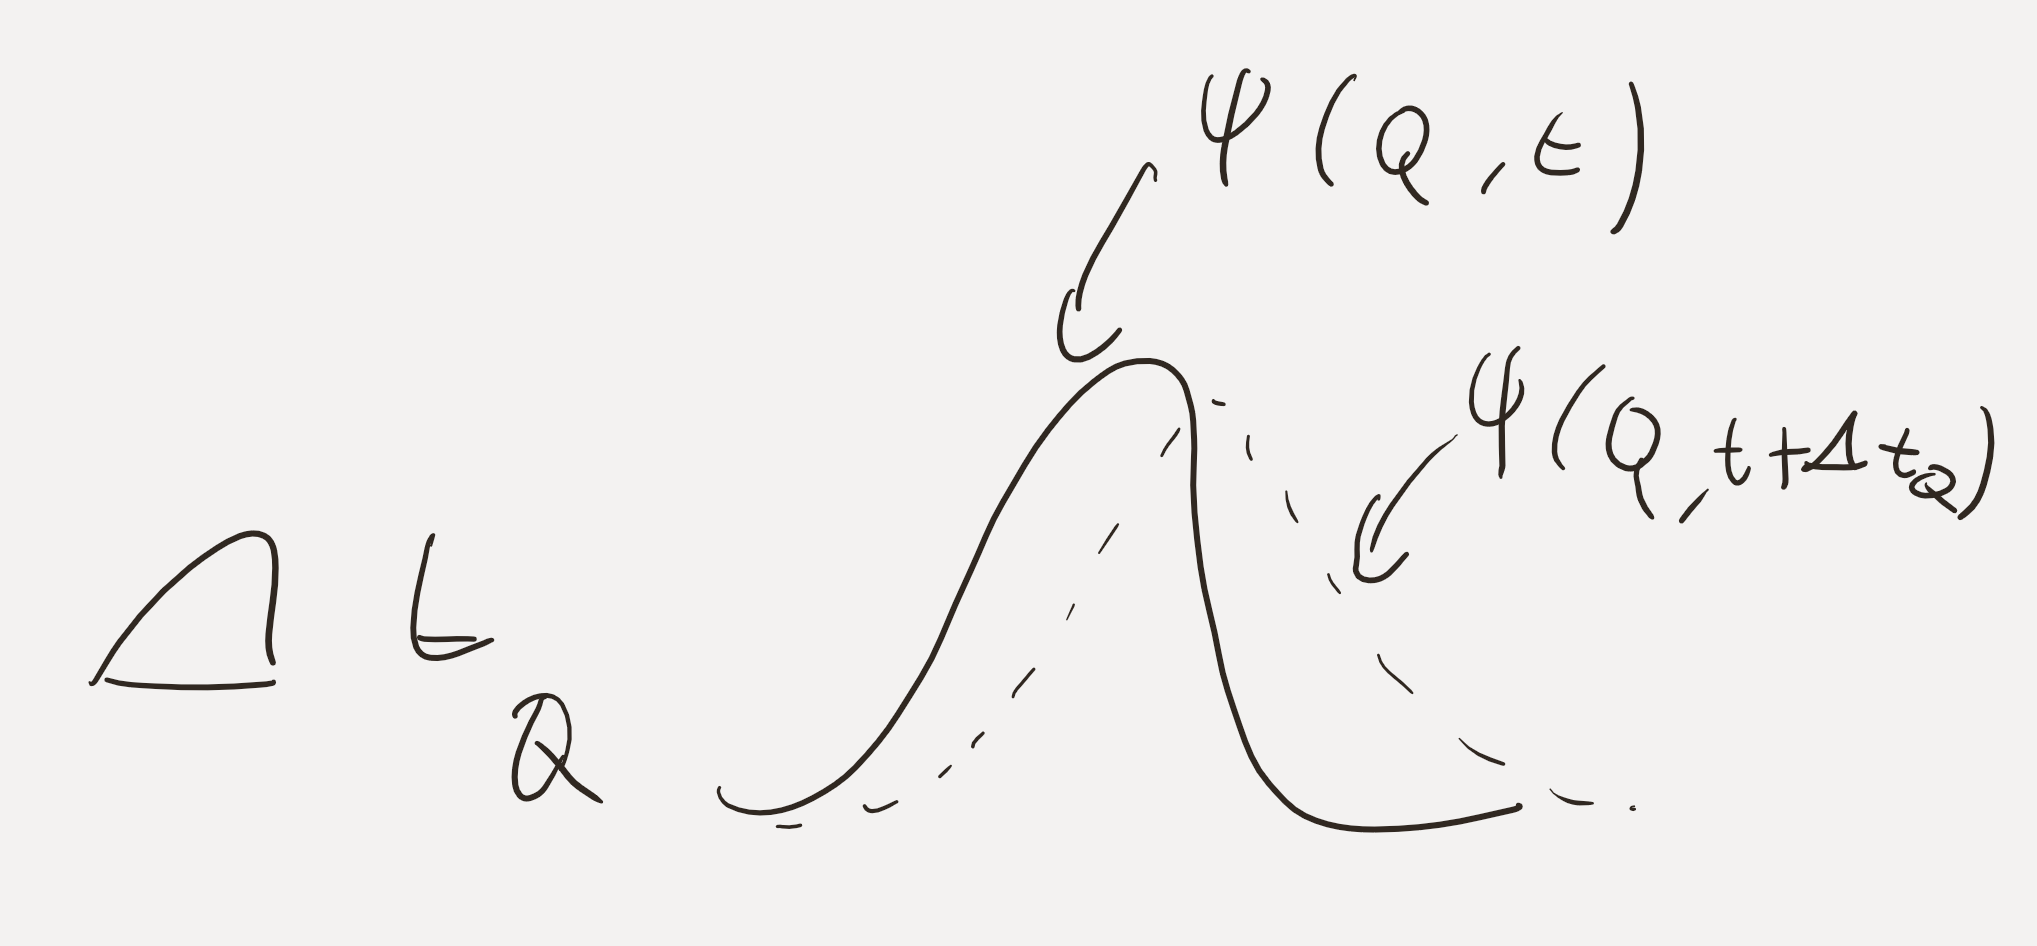
\includegraphics[width = 0.6 \textwidth]{Lecture18/1.png}

\section{Today}

\begin{itemize}
    \item Finish off discussion of the uncertainty relations and end chapter 3. 
    \item Begin our treatment of particle physics in three dimensions. 
\end{itemize}

\hfill

\subsection*{Recall:}

$$\frac{d}{dt} \braket{\hat{Q}} = \frac{i}{\hbar} \braket{[\hat{H}, \hat{Q}]}$$

together with $$\sigma_H^2 \sigma_Q^2 \geq \left( \frac{1}{2i} \braket{[\hat{H}, \hat{Q}]} \right)^2$$

$$\sigma_H^2 \sigma_Q^2 \geq \left( \frac{1}{2i} \frac{\hbar}{i} \frac{d \braket{\hat{Q}}}{dt} \right)^2$$

$$\sigma_H \sigma_Q \geq \left|  \frac{\hbar}{2} \frac{d \braket{\hat{Q}}}{dt} \right|$$

\subsection*{Reflect on our results comparing $\sigma_p^2 \sigma_E^2$  for free particles and for particles in a harmonic potential:}

For a particle in a harmonic potential: $\sigma_p^2 \sigma_E^2 \geq \frac{\hbar^2}{4} k^2 \braket{\hat{x}}^2 (t)$, and for a free particle, $\sigma_p^2 \sigma_E^2 \geq 0$. This is as deduced from the generalized uncertainty relation. 


Free particle: Key point is that it is possible that there exist states for which the variances of both $p$ and $E$ can be arbitrarily close to zero (e.g. their shared eigen bases), but not all valid free particle states have zero variances in $p$ and $E$. 


Harmonic oscillator: key points are that:
\begin{enumerate}
    \item Product of variances is state dependent, and in general not equal to zero (consistent with not sharing common eigen states)
    \item Since this product is state dependent, it is also in general time-dependent
    \item Beyond this, not so easy to interpret from the generalized uncertainty relation alone
\end{enumerate}

\section{Discuss: Energy-time analysis}

Does the energy-time analysis of the product of variances add any useful insight to this comparison of the free particle and the oscillator results for $\sigma_p \sigma_H$?

$$\sigma_p \sigma_H \equiv \sigma_p \sigma_E \geq \frac{\hbar}{2} \left| \frac{d \braket{\hat{p}}}{dt} \right|$$

For the free particle, $|\hat{p}, \hat{E}| = 0$:

\begin{itemize}
    \item Therefore $\frac{d \braket{\hat{p}}}{dt} = 0$, always
    \item Therefore momentum is conserved
    \item $\hat{p}, \hat{E}$ have a shared set of eigen states
    \item The product of their variances can be arbitrarily close to 0
\end{itemize}

For the harmonic oscillator, $[\hat{p}, \hat{E}] \neq 0$, $[\hat{p}, \hat{E}] = -i\hbar k \braket{\hat{x}} (t)$

\begin{itemize}
    \item Therefore  $\frac{d \braket{\hat{p}}}{dt} \neq 0$ in general, implying a net force can be exerted on the particle
    \item Momentum is \textbf{not necessarily conserved}
    \item $\hat{p}, \hat{E}$ \textbf{do not share a common set of eigen states}
    \item The product of their variances is state and in general time dependent:
    
    $$\sigma_p^2 \sigma_E^2 \geq \frac{\hbar^2}{4} k^2 \braket{\hat{x}} (t)$$
\end{itemize}

If momentum is changing rapidly (relative to variance of momentum), then this implies that there must be quite a bit of uncertainty in measurements of the energy at that time.  

Think through for a wavepacket that mimics the classical motion of a particle in a harmonic potential…(momentum zero when probability density close to classical turning points, and a maximum in centre, when probability distribution is symmetric).  So rate of change of momentum large at extremes, and zero in middle…is this consistent with our formula?


\subsection{Polls}

\begin{enumerate}
    \item  If the particle was in a stationary state of the harmonic oscillator, its momentum would be time-dependent (T/\textbf{F})
    \item  If the particle was in a stationary state of the harmonic oscillator, the product of the variances $\sigma_p^2 \sigma_E^2 \geq 0$ (\textbf{T}/F)
    \item  If the particle was in a stationary state of the harmonic oscillator, the product of the variances  $\sigma_p^2 \sigma_E^2 = 0$ (\textbf{T}/F)
    \item If the particle was in a wavepacket state comprising several harmonic oscillator stationary states, that closely mimicked the classical oscillatory motion of a particle in a harmonic potential,  $\sigma_p^2 \sigma_E^2 \geq 0$ periodically, when it was moving past the centre of the potential well, and  $\sigma_p^2 \sigma_E^2 \geq \frac{\hbar^2}{4} k^2 \braket{\hat{x}}^2_{\{max\}}$ periodically, when it was at its maximum excursion points $\pm \braket{\hat{x}}_{\{max\}}$  (\textbf{T}/F)
    \item The energy-time uncertainty relation helps explain the basic generalized uncertainty relation in this particular problem, because the product of variances must exceed the instantaneous force acting on the particle, which directly tells you how rapidly the momentum must be changing (\textbf{T}/F) \footnote{can formulate by estimating $\Delta p~ \Delta t_E$ Force, where $\Delta t_E$ is approx. $\hbar/2/\sigma_E$, motivated by “characteristic frequency” in quantum problems roughly goes as the difference in energy (cf 2 state dynamics)}

\end{enumerate}

\section{Particles moving in 3D: General considerations}

What is the fundamental change in dynamical variables that must be made in going from the 1D to the 3D SE for a single, non-relativistic electron in a time-invariant potential?

$$x \rightarrow \vec{R}, p \rightarrow \vec{p}$$

%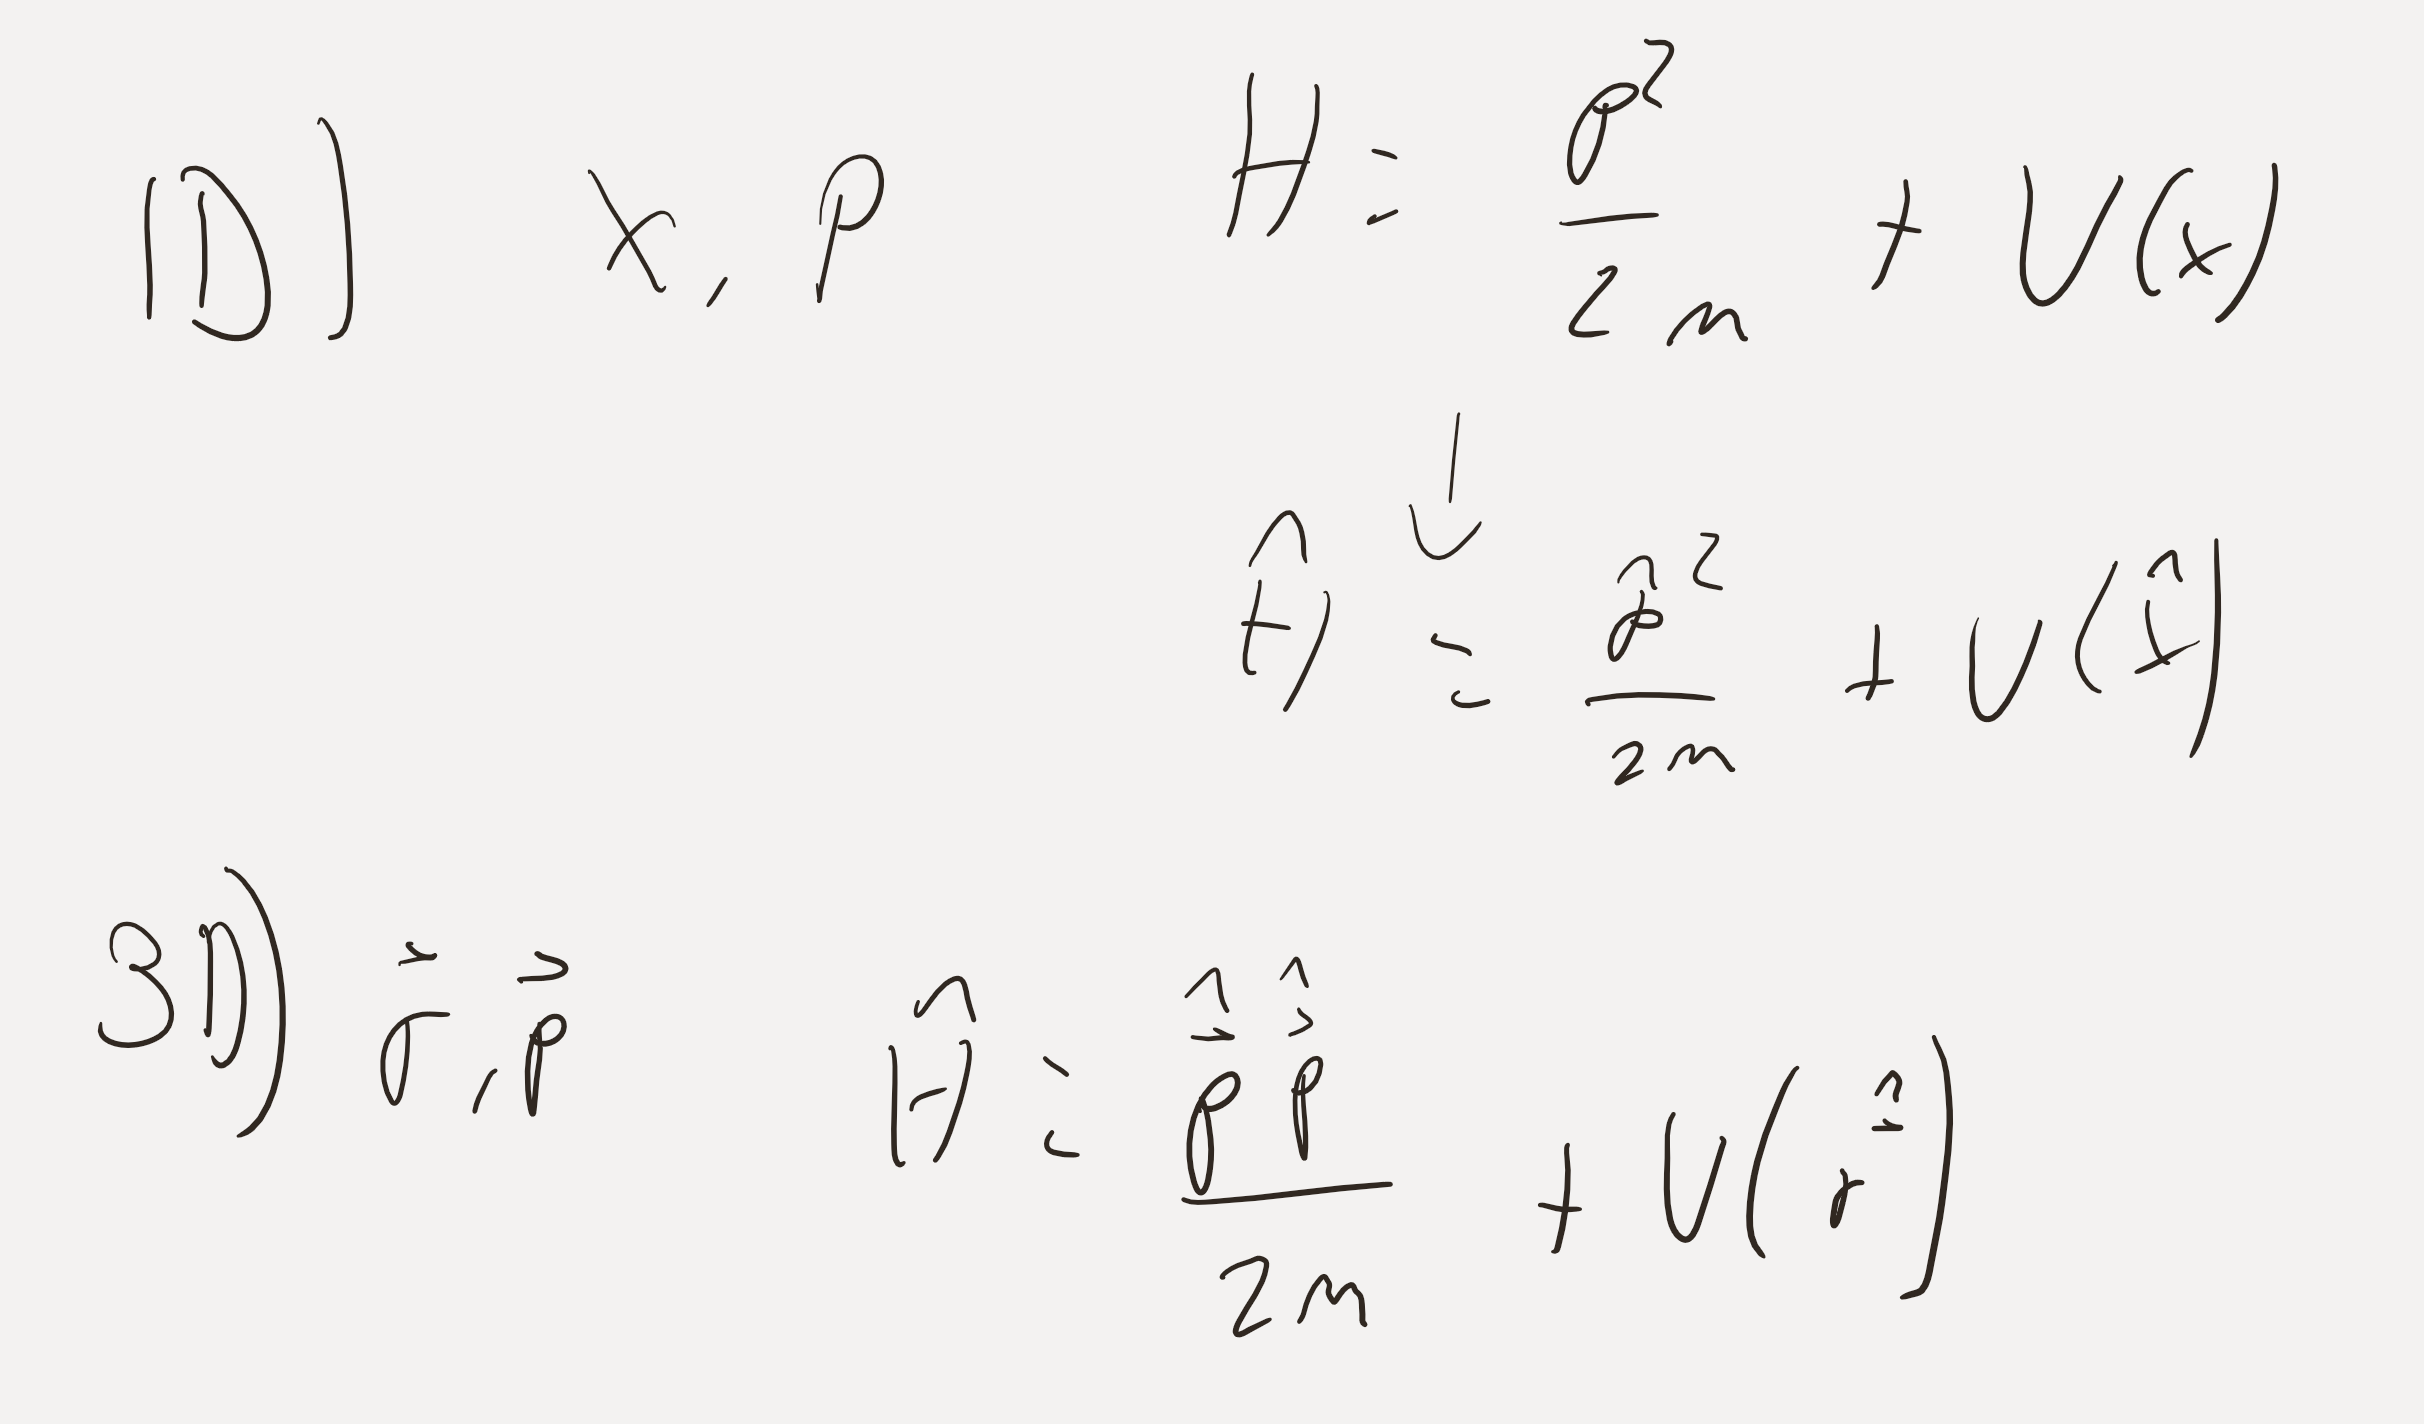
\includegraphics[width = 0.8 \textwidth]{Lecture18/2.png}

In 1 dimension, $x,p$ $\longrightarrow H = \frac{p^2}{2m} + V(x)$, and $\hat{H} = \frac{\hat{p}^2}{2m} + v(\hat{x})$

Hence, in 3 dimensions, $\hat{r}, \hat{p}$ $\longrightarrow \hat{H} = \frac{\hat{\vec{p}} \hat{\vec{p}}}{2m} + V(\hat{\vec{r}})$

What is a subtle implication of this change of dimension (not peculiar to quantum mechanics per se)?  (eg. what new, interesting “observables” can one define?)

More degrees of freedom, and more symmetries: e.g. rotation, angular momentum as observables, and, related, rotational symmetries.  


\section{Exercise 1}

A1) What is the classical equation that describes the total energy of a non-relativistic electron in 3D, using vector notation for the dynamical variables?

Put hats on p and r


A2) Convert this expression to a basis-agnostic quantum mechanical Hamiltonian operator.

divergence, dot divergence, = $\nabla^2$, can get rid of the  $\hat{}$ on r in $V(\vec r)$.  To go any further, now must choose a 3D vector basis (distinct from QM basis!!).  What was our only choice in 1D?  (origin and direction/sense of x).

A3) Express the 3D electron Hamiltonian operator in the position basis, $\hat{\vec{r}}$.  What additional choices do you have to make at this point?  Why didn't we worry about this issue in 1D?

In position basis, differential form of $\hat{H}$:

$$\hat{\vec{p}} \text{ in the position basis } = -i \hbar \left( \frac{d}{dx} \hat{i} \frac{d}{dy} \hat{j} \frac{d}{dz} \hat{k} \right) = -i \hbar \hat{\vec{\nabla}}_{\vec{r}}$$

$$\hat{H} = \frac{-\hbar^2}{2m} \left( \frac{\partial^2}{\partial x^2} + \frac{\partial^2}{\partial y^2} + \frac{\partial^2}{\partial z^2} \right) + V(\vec{r})$$

\begin{enumerate}
    \item Solve the TISE (in general functions)
    \item Use boundary conditions to restrict general solution to a set of eigen functions $\{\psi_n(x)\}$ and corresponding eigen values $\{E_n\}$
    \item Use initial wavefunction $\Psi(x,t=0)$ to get $\{c_n\}$; $\Psi(x,t=0) = \sum_n c_n \psi_n(x)$
\end{enumerate}

\subsection{Example 2}

Solve the 3D time independent SE for a potential that is infinite everywhere except inside a cube with one corner at the origin, (0,0,0), and one at (a,a,a).


\begin{itemize}
    \item Write correct time-independent SE $(- \nabla^2 \psi = E\psi)$
    \item Show $e^{i \vec k \cdot \vec r}$ is a valid form of the general solution before using BCs
    \item Write out as product of 3 functions of x, y, and z
\end{itemize}

Note that BCs are such that can easily use them with this form of the general solution (what would be the issue if it were a sphere rather than a cube?


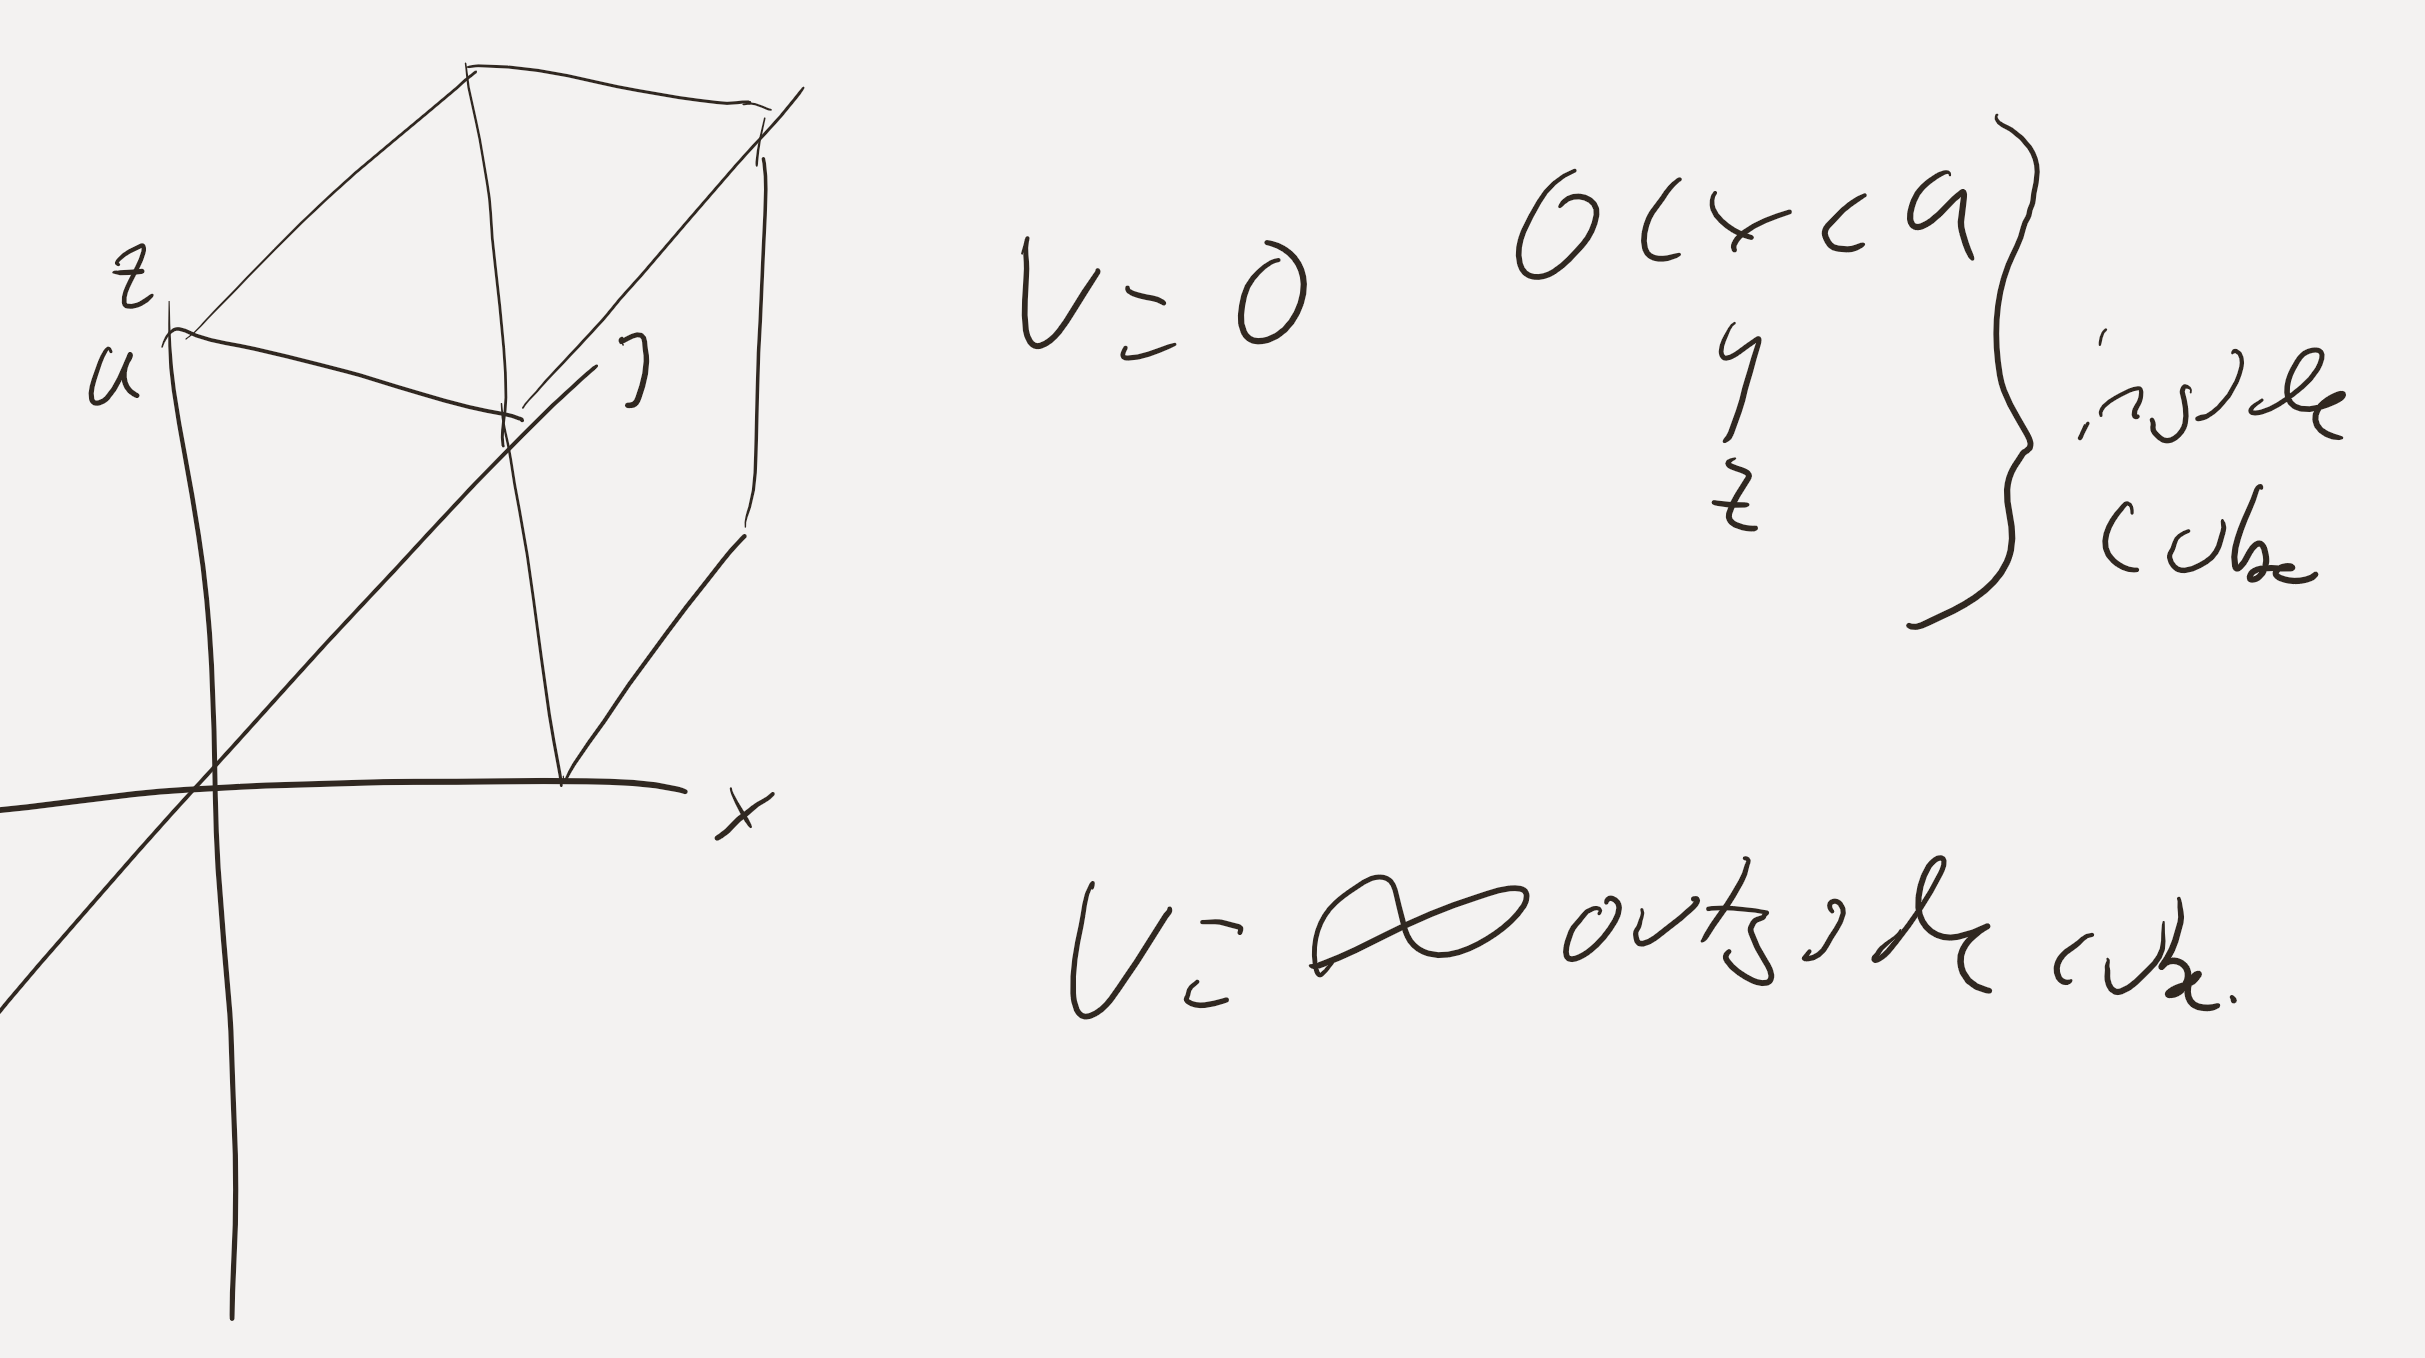
\includegraphics[width = 0.8 \textwidth]{Lecture18/3.png}

$$- \frac{\hbar^2}{2m} \frac{1}{\psi_x(x)} \frac{\partial^2 \psi_x(x)}{\partial x^2} - \frac{\hbar^2}{2m} \frac{1}{\psi_y(y)} \frac{\partial^2 \psi_y(y)}{\partial x^2}    - \frac{\hbar^2}{2m} \frac{1}{\Psi_z(z)} \frac{\partial^2 \psi_z(z)}{\partial z^2} = E$$

This can only be true if they are equal to some constant - $E_x$ for the x portion, $E_y$ for the y portion, etc. 

Boundary conditions:

$$\psi_x(0) = \psi_x(a) = \psi_y(0) = \psi_y(a) = \psi_z(0) = \psi_z(a) = 0$$

$$\Psi(\vec{r}) \propto \sin \left( \frac{n_x \pi x}{a} \right) \sin \left( \frac{n_y \pi y}{a} \right) \sin \left( \frac{n_z \pi z}{a} \right)$$

\begin{align*}
    n_x = 1,2,3...
    n_y = 1,2,3...
    n_z = 1,2,3...
\end{align*}

Where $n_x, n_y, n_z$ have no inherent correlation with each other. 

$$\therefore E_{n_x, n_y, n_z} = E_x + E_y + E_z = \frac{\hbar^2}{2m} \frac{\pi^2}{a^2} \left( n_x^2 + n_y^2 + n_z^2 \right)$$





\end{document}
